\chapter{Passiv Radar Setup}
\section{Einführung}
\section{Hardware}
\subsection{ADALM-Pluto SDR}
Bei dem hier verwendeten SDR handelt es sich um ein ADALM
PLUTO SDR. Der Hauptgrund, warum sich in diesem Versuchsaufbau für dieses Gerät entschieden wurde ist die Bandbreite dieses Gerätes die bei bis zu 20 MHz liegt. Die Bandbreite des Signals was hier für Passiv Radar verwendet beträgt nämlich 5MHz was einige SDR nicht aufbringen können.  Aufs weitere besitzt das SDR eine Frequenz Abdeckung von 325 MHz bis zu 3.8 MHz. Die weiteren Daten können in der Tabelle abgelesen werden.

\subsubsection{Synchronität}
Zur Aufnahme des Referenzsignals als auch des reflektierten Signals werden jeweils ein Pluto-SDR benötigt, diese zwei müssen nun synchron betrieben werden. Dies wird erreicht durch Daisy Chaining  der beiden Uhren der SDRs und einer externen Uhr. Abbildung zeigt dann den fertigen Aufbau der Beiden SDRs und im Schaltplan in Abbildung ist zur erkennen wie die Uhr der jeweiligen SDRs aufgebaut ist.
\subsection{Antenne}
In diesem Aufbau werden zwei Antennen die für DVB-T gedacht sind verwendet. Die Antenne ist ein Yagi Antenne mit 43 Elementen wie man im Abbildung /ref{antenne} sieht die im Frequenzbereich von 470 bis 862 MHZ arbeitet, was für unseren Anwendungsfall sehr gut geeignet ist.Die weiteren Daten zur Antenne stehen in der Tabelle /ref{table:antenne}.

\begin{table}
    \centering
        \begin{tabular}[h]{rl}
            Antenne         & SKT SL43-01 UHF 43            \\
            Antennengewinn  & 11..13 dB                     \\
            Frequenzbereich & 470-862 MHz                   \\
            Halbwertsbreite & horiz. 30...40°/ver. 35...50° \\
        \end{tabular}
    \caption{Daten der SKT SL43-01 UHF 43 Antenne}\label{table:antenne}
\end{table}

\begin{figure}
    \centering
    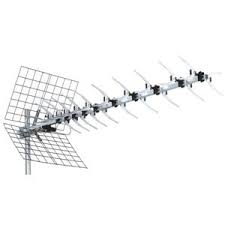
\includegraphics[width=\textwidth]{images/antenne.png}
    \caption{SKT SL43-01 UHF 43 Antenne}\label{antenne}
\end{figure}
\section{Signal}
\subsection{Aufbau von LTE}
\subsubsection{PSS}
\subsubsection{SSS}
\section{Software}

Nachfolgend soll nun die verwendete Softwaresuite erläutert werden. Dazu wird zunächst die zur Aufnahme genutzte Lösung beschrieben. Anschließend wird näher auf die eigens entwickelte Signalverarbeitungskette eingegangen.

\subsection{Aufnahme}

Um Daten vom PlutoSDR zu empfangen bedarf es einer Bediensoftware um den Empfangsprozess zu steuern. Zahlreiche solcher SDR-Anwendungen existieren auf dem Markt, viele davon Open-Source oder als Freeware erhältlich. Der Hersteller selbst, Analog Devices, bietet ein low-level Treiberpaket names \emph{libiio} (der Name setzt sich zusammen aus dem Unix typischen lib-Präfix für \emph{library} und dem Akronym iio---%
% cspell:disable-next-line
\textbf{i}ndustrial \textbf{i}nput/\textbf{o}utput---%
steht) an. Mit diesem ist es möglich lokal-, über USB- oder Netzwerk verbundene ADCs und FPGAs von Analog Devices zu steuern. Das Treiberpaket beinhaltet dabei einige Kommandozeilenanwendungen mit denen angeschlossene Geräte enumeriert, einzelne Register gelesen und beschrieben und die Firmware ak­tu­a­li­sie­rt werden können. Darüber hinaus kann über eine API, die Teil der namensgebenden libiio Bibliotheksdatei ist, auf Geräte zugegriffen werden.

Es ist diese API an der die meisten SDR-Anwendungen ansetzten. Welche Funktionen der Hardware dann genau nutzbar sind, hängt von der jeweiligen Anwendung ab. Für die Durchführung dieses Projekts würde sich dabei für die Anwendung SDRangel\footnote{Homepage: \url{https://bit.ly/sdrangel}} von Edouard Griffiths entschieden. Abbildung~\ref{fig:sdrangel_screenshot} zeigt die graphische Oberfläche der Anwendung. Die Software unterstützt das Darstellen und Aufzeichnen von IQ-Rohdaten in einem eigenen Dateiformat. Die Möglichkeit der Live-Darstellung der Daten in Frequenz- und Wasserfalldiagramm hat sich in den Messkampagnen als äußerst hilfreich erwiesen.

\begin{figure}[htb]
    \centering
    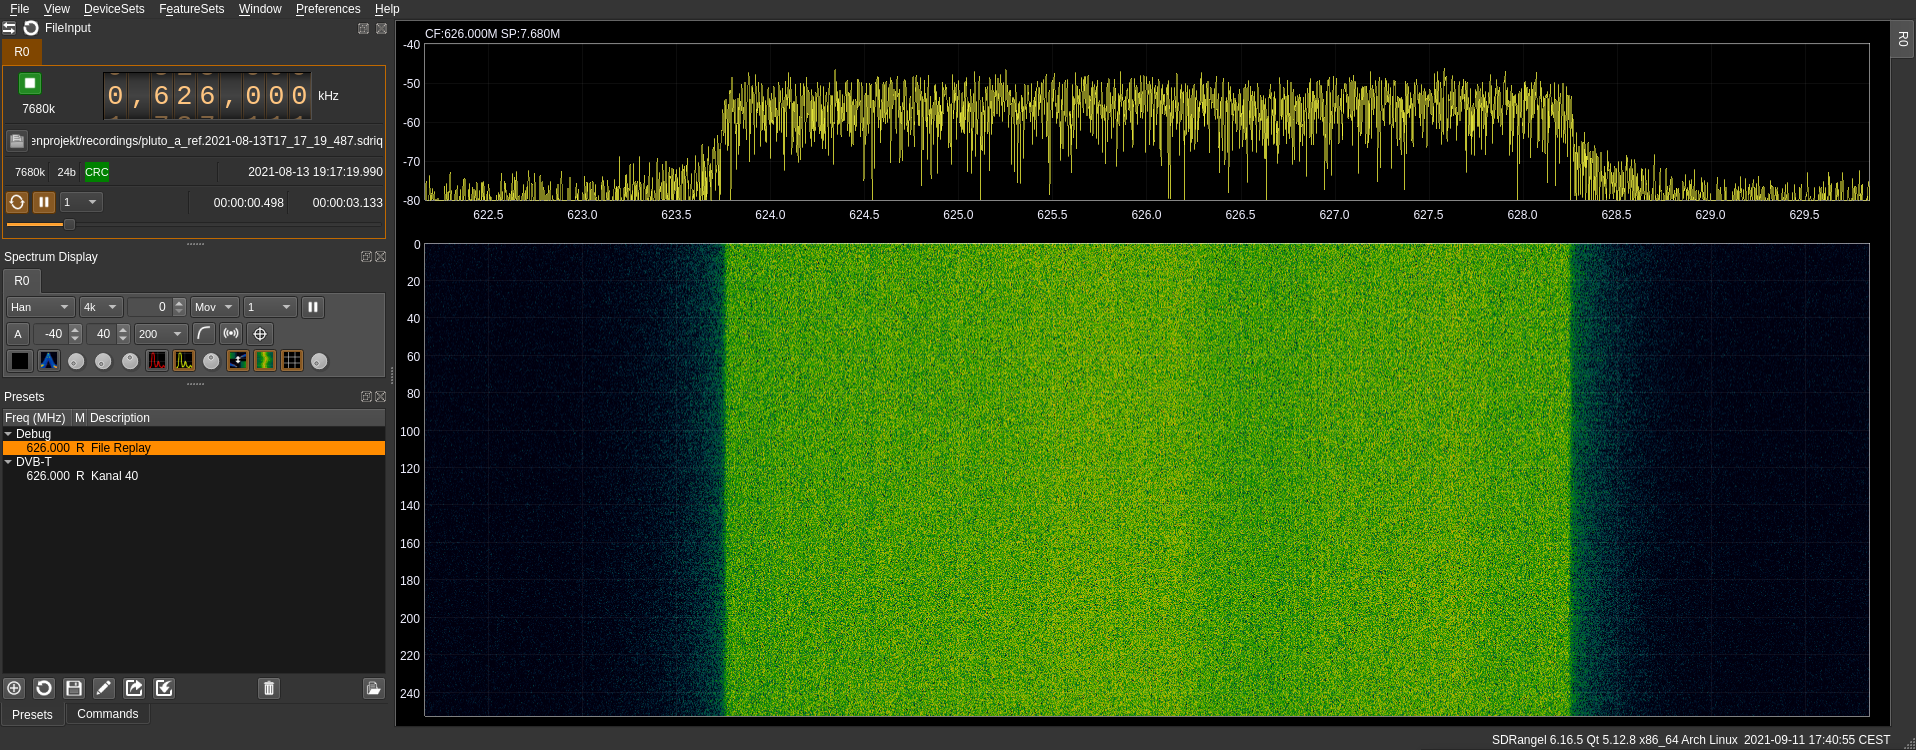
\includegraphics[width=\textwidth]{images/sdrangel.png}
    \caption{SDRangel im Replay-Modus einer zuvor angefertigten Messung.}\label{fig:sdrangel_screenshot}
\end{figure}

Da es sich hierbei um Open-Source-Software handelt, konnten benötigte Funktionen oder Bugfixes\footnote{Liste aller Änderungen: \url{https://bit.ly/sdrangel-pr}} direkt selbst implementiert werden und sind anschließend ins Projekt zurück geflossen. So wurde ein Bugfix zur parallelen Nutzung zweier PlutoSDR erstellt, eingereicht und in den Hauptentwicklungszweig des Ursprungsprojekts aufgenommen.

\subsection{Signalverarbeitung}

Die Signalverarbeitungskette stellt den essenziellen Teil dieser Projektarbeit dar. Bereits zu beginn des Projekts wurde sich dafür entschieden, diese weitestgehend in Python zu implementieren. Als Grundlage für mathematische Operationen dient dabei die numerische Mathematikbibliothek \emph{NumPy}. Zusätzlich wird vereinzelt auf Funktionen der \emph{SciPy-Signal} (Grundbausteine für Funktionen der Signalverarbeitung) oder \emph{CuPy} (GPU-beschleunigte Implementierung der NumPy-Funktionen) Bibliotheken zurückgegriffen. Ziel war es, sich eng vertraut mit den Aspekten der Signalverarbeitung zu machen, und weniger auf vorbereitete Funktionen zurückzugreifen; ohne deren Details zu verstehen. Der Entwicklungsprozess ließ sich dabei grob in zwei Schritte unterteilen. Zunächst wurden Algorithmen prototypisch in Form von Jupyter Notebooks implementiert und getestet. Hier konnten die Methoden und Algorithmen interaktiv entworfen werden, bevor sie im zweiten Schritt in solide und testbare Python Module ausgegliedert wurden.

Die so entstandene Signalverarbeitungskette ist in Abbildung~\ref{fig:signal_processing_chain} gezeigt. Die Direkt- und Echosignale werden über zwei getrennte Kanäle aufgezeichnet. Die beiden Empfänger sind dabei am Wandler phasen- und frequenzkohärent getaktet. Durch die Wandler entsteht ein analytisches Zeitsignal, bestehend aus einer in- und einer \(90^\circ \) verschobenen Phasenkomponente %
% cspell:disable-next-line
(engl.\@ \textbf{I}n-phase und \textbf{Q}uadrature-phase). %
Nach der Wandlung werden diese Daten per USB-Schnittstelle an einen Computer übertragen und dort aufgezeichnet. Dabei ist anzumerken, dass bereits durch die USB-Übertragung jegliche Synchronität der beiden Kanäle verloren geht. Um dem entgegen zu wirken, wird im Dateikopf jeder Aufzeichnung ein Millisekunden genauer Zeitstempel hinterlegt. Da jedoch weder das Betriebssystem noch die Aufnahmesoftware harte Echtzeit unterstützt ist auch hier von mehreren Millisekunden Jitter auszugehen. Um dies zu kompensieren wurde eine Synchronisierungsschnittstelle entworfen, die versucht, die beiden Datenströme zeitlich anzugleichen. Dazu wird zunächst eine grobe Angleichung mittels Zeitstempel aus der Aufzeichnung vorgenommen, anschließend wird versucht über die im LTE Signal enthaltenen Synchronisierungssequenzen eine OFDM-Symbol genaue Synchronisierung herzustellen. So entstehen zwei in Zeit, Frequenz und Phase synchronisierte Datenströme, die für die weitere Prozessierung verwendet werden.

Die mitführung des Referenzkanals ermöglicht grobe Clutter Suppression mittels \emph{CLEAN} Algorithmus~\cite{Kulpa2019}. Dazu soll im Folgenden genauer auf die Kernelemente \emph{CAF} und \emph{CLEAN} eingegangen werden. Finales Ergebnis der Prozesskette ist eine von Clutter bereinigte Range-Doppler Matrix. Zukünftige Arbeiten könnten an dieser Stelle ansetzen und die Informationen aus der Range-Doppler Matrix zur Alarmerzeugung nutzen.

\begin{figure}[htb]
    \centering
    \begin{tikzpicture}[
            flow node/.style={
                    draw,
                    fill=blue!20,
                    rounded corners,
                    minimum height=2em,
                    minimum width=5cm,
                },
            every edge quotes/.style={
                    fill=white,
                    rounded corners,
                    fill opacity=0.8,
                    text opacity=1,
                    font=\scriptsize,
                }
        ]
        \coordinate (origin) at (0,0);

        \node (pluto_a) [flow node, left=0.5cm of origin, anchor=east] {PlutoSDR A};
        \node (pluto_b) [flow node, right=0.5cm of origin, anchor=west] {PlutoSDR B};

        \node (antenna_a) [bareRXantenna, above=1.5cm of pluto_a]{Rx A};
        \node (antenna_b) [bareRXantenna, above=1.5cm of pluto_b]{Rx B};

        \node (recording_ref) [flow node, below=1.5cm of pluto_a, anchor=north] {Aufzeichnung (Ref.)};
        \node (recording_surv) [flow node, below=1.5cm of pluto_b, anchor=north] {Aufzeichnung (Surv.)};

        \node (parser_ref) [flow node, below=1.5cm of recording_ref, anchor=north] {Parser};
        \node (parser_surv) [flow node, below=1.5cm of recording_surv, anchor=north] {Parser};

        \path let \p1=($(parser_ref.south)!0.5!(parser_surv.south)$) in node (sync) [flow node, below=1.5cm of (\p1), anchor=north] {Synchronisation};

        \node (caf) [flow node, below=1.5cm of sync, anchor=north] {CAF};

        \node (clean) [flow node, right=1.5cm of caf, anchor=west] {CLEAN};

        \node (display) [flow node, below=1.5cm of caf, anchor=north] {Anzeige};

        \draw (antenna_a) -- (pluto_a);
        \draw (antenna_b) -- (pluto_b);
        \path (pluto_a) edge [->,"IQ Rohdaten"] (recording_ref);
        \path (recording_ref) edge [->,"\directory{reference.sdriq} Datei"] (parser_ref);
        \path (parser_ref) edge [->,"Zeitsignal"] (sync);
        \path (pluto_b) edge [->,"IQ Rohdaten"] (recording_surv);
        \path (recording_surv) edge [->,"\directory{surveillance.sdriq} Datei"] (parser_surv);
        \path (parser_surv) edge [->,"Zeitsignal"] (sync);
        \path (sync) edge [->,"(2x) Sync. Zeitsignal"] (caf);
        \path let \p1=($(caf.east) + (0,0.2cm)$), \p2=($(clean.west) + (0,0.2cm)$) in (\p1) edge [->,"Range-Doppler Matrix" {right,rotate=40}] (\p2);
        \path let \p1=($(clean.west) - (0,0.2cm)$), \p2=($(caf.east) - (0,0.2cm)$) in (\p1) edge [->,"Bereinigte Zeitsignale" {right,rotate=-40}] (\p2);
        \path (caf) edge [->,"Range-Doppler Matrix"] (display);
    \end{tikzpicture}
    \caption{Schematische Darstellung der Signalverarbeitungskette.}\label{fig:signal_processing_chain}
\end{figure}

\subsubsection{Ambiguity Funktion}\label{sct:ambiguity_function}
\subsubsection{Clean Algorithmus}
